\chapter{Design af brugergrænsefladen}
\label{Design_G}
Dette kapitel beskriver brugergrænsefladen samt de beslutninger, som ligger bag. Alle vores papermockups og endelige skærmbilleder findes i appendix \ref{App_GUI}.

\section{Brugergrænsefladens udvikling og udseende}
\label{Design_G_Development}
\begin{figure}[h!]
  \centering
    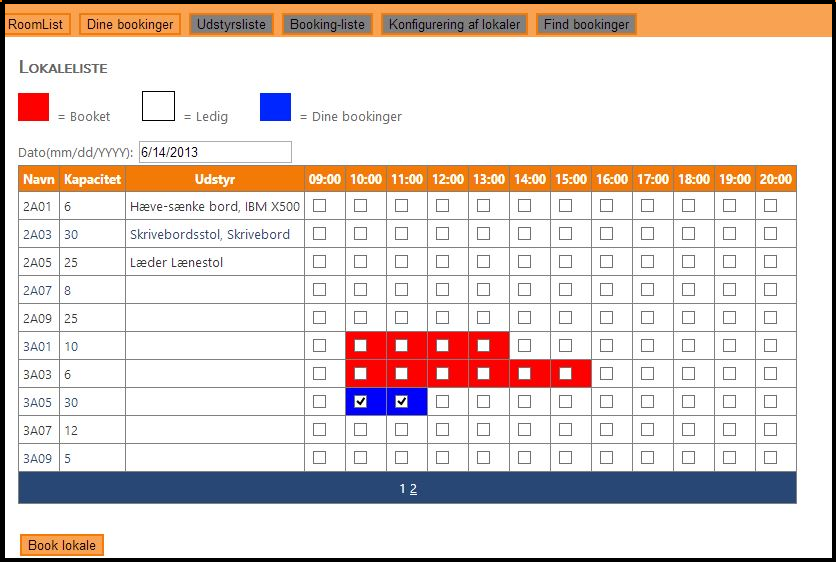
\includegraphics[width=0.85\textwidth]{Appendix/GUI-Prototype/DigitalMockup/GridEksempel}
  \caption{Skærmbilledet til booking af lokaler}
\label{Design_G_Development_FinalGrid}
\end{figure}

Figur \ref{Design_G_Development_FinalGrid} er det første skærmbillede man ser, når programmet starter. Det er en liste over lokaler, som viser, hvilke tidsrum lokalerne er til rådighed.
\\For at booke et lokale markerer man tiderne i checkboksene, der hører til det ønskede lokale og trykker "Book lokale". Hvis man ikke er logget ind, bliver man bedt om at logge ind, før man kan fortsætte.
\\Det har været vores mål, at brugeren skal have adgang til så meget information, som det er muligt at give, uden at brugeren logger ind.

\begin{figure}[h!]
  \centering
    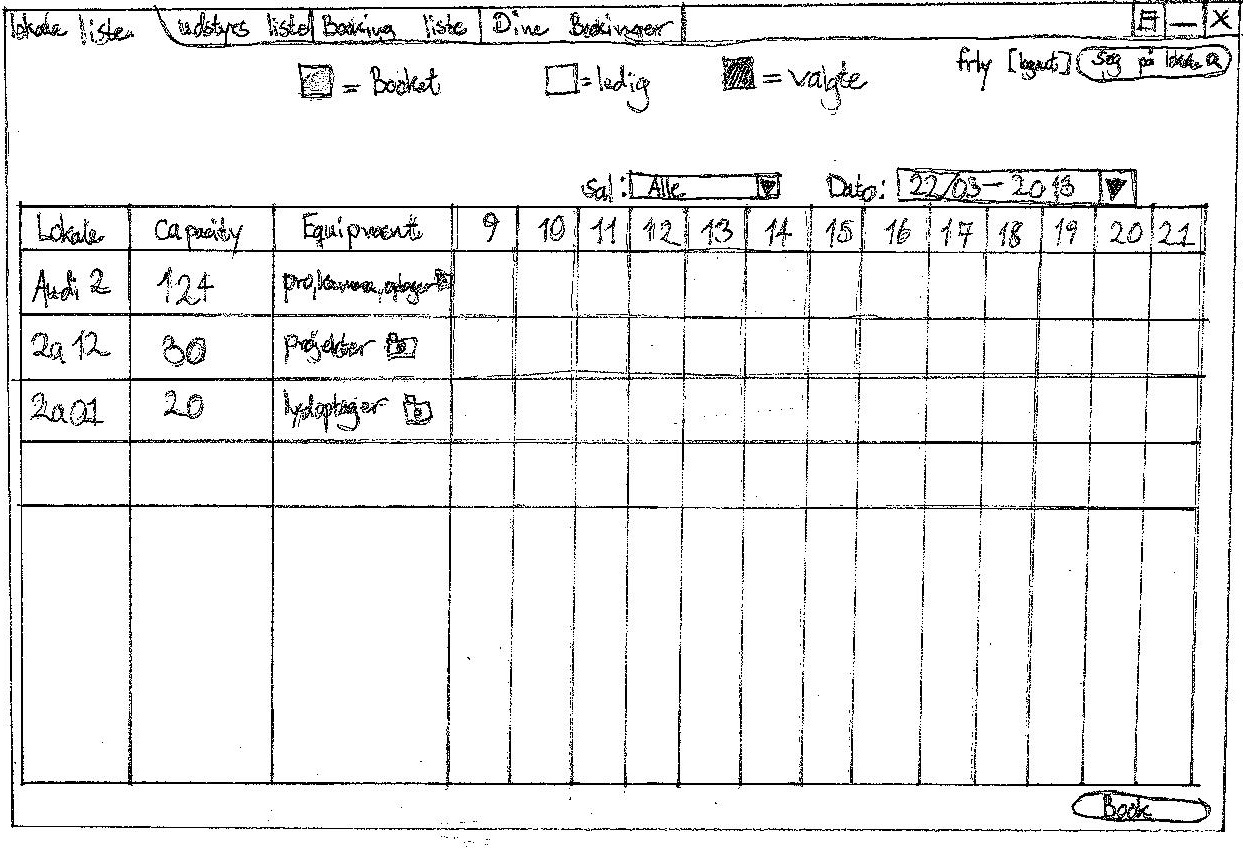
\includegraphics[width=0.9\textwidth]{Appendix/GUI-Prototype/PaperMockup/LokaleListe_001}
  \caption{Første udgave af skærmbilledet til booking af lokaler}
\label{Design_G_Development_FirstGrid}
\end{figure}

Vores første mockup af skærmbilledet til booking af lokaler (figur \ref{Design_G_Development_FirstGrid}) havde et gitter, hvor hver række var et lokale og tiderne var kolonner. Man skulle klikke i et felt for at vise, at man ønskede at booke på et bestemt tidspunkt. Vores usability test viste dog, at det ikke var en intuitiv måde at vælge tidspunkter på, så vi tilføjede checkbokse til gitteret.

\begin{figure}[h!]
  \centering
    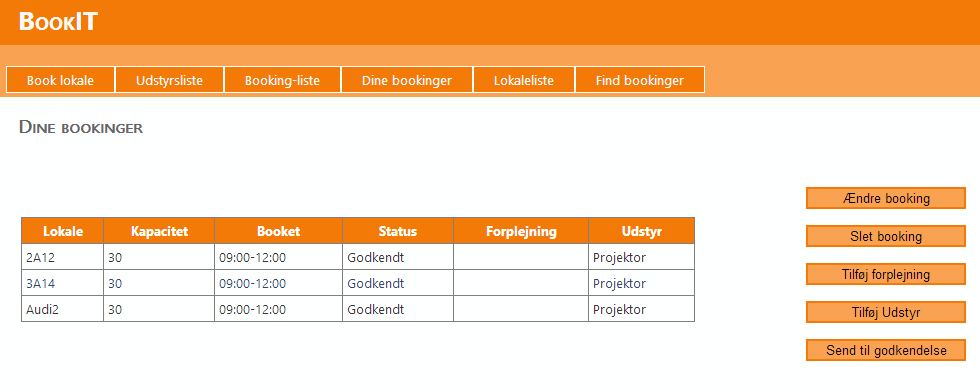
\includegraphics[width=0.9\textwidth]{Appendix/GUI-Prototype/DigitalMockup/DineBookinger}
  \caption{Skærmbilledet til visning brugerens bookinger}
\label{Design_G_Development_YourBookings_Final}
\end{figure} 

Når man har valgt lokale og tidsrum, trykker man "Book lokale". Dette redirecter brugeren til skærmbilledet "Dine Bookinger", som viser en liste over brugerens bookinger (se figur \ref{Design_G_Development_YourBookings_Final}). 
\\Hvis man vælger en booking i listen og trykker "Ændre Booking", navigeres der til lokalelisten, hvor man kan ændre sin booking ved at tilføje/fjerne markeringer i checkboksene. 
\\Hvis man trykker "Tilføj Forplejning", vises "Forplejningsskærmbilledet".

\begin{figure}[h!]
  \centering
    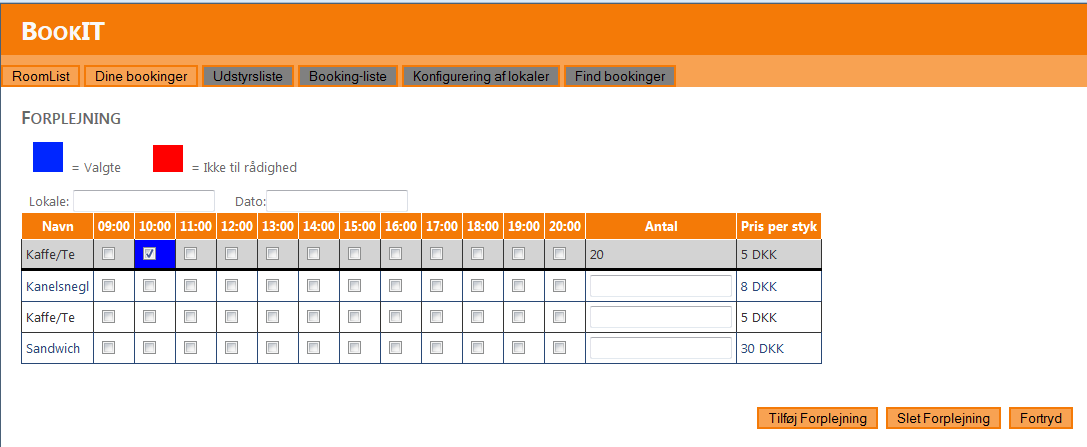
\includegraphics[width=0.9\textwidth]{Appendix/GUI-Prototype/DigitalMockup/Forplejning}
  \caption{Skærmbilledet til bestilling af forplejning}
\label{Design_G_Development_Forplejning_Final}
\end{figure} 

Figur \ref{Design_G_Development_Forplejning_Final} viser det endelige skærmbillede til valg af forplejning. For at tilføje forplejning til en booking skal man markere den tid, man gerne vil have forplejningen leveret samt angive, hvor mange/meget af forplejningstypen, man gerne vil bestille.
\\Vi fokuserede på at designe skærmbilledet på samme måde, som vi havde designet skærmbilledet til lokalelisten. Det samme gælder for skærmbilledet til tilføjelse af udstyr til en booking (se figur \ref{App_GUI_final_BookEquip} i appendix).

\subsection{Bookingliste}
\begin{figure}[h!]
  \centering
    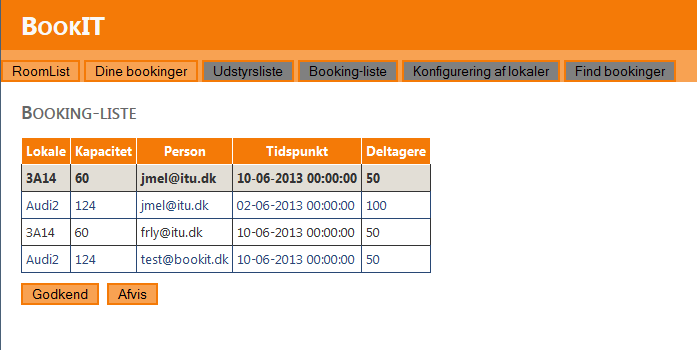
\includegraphics[width=0.8\textwidth]{Appendix/GUI-Prototype/DigitalMockup/BookingListe}
  \caption{Skærmbilledet til godkendelse og afvisning af bookinger}
\label{Design_G_Development_BookingListe_Final}
\end{figure} 

\begin{figure}[h!]
  \centering
    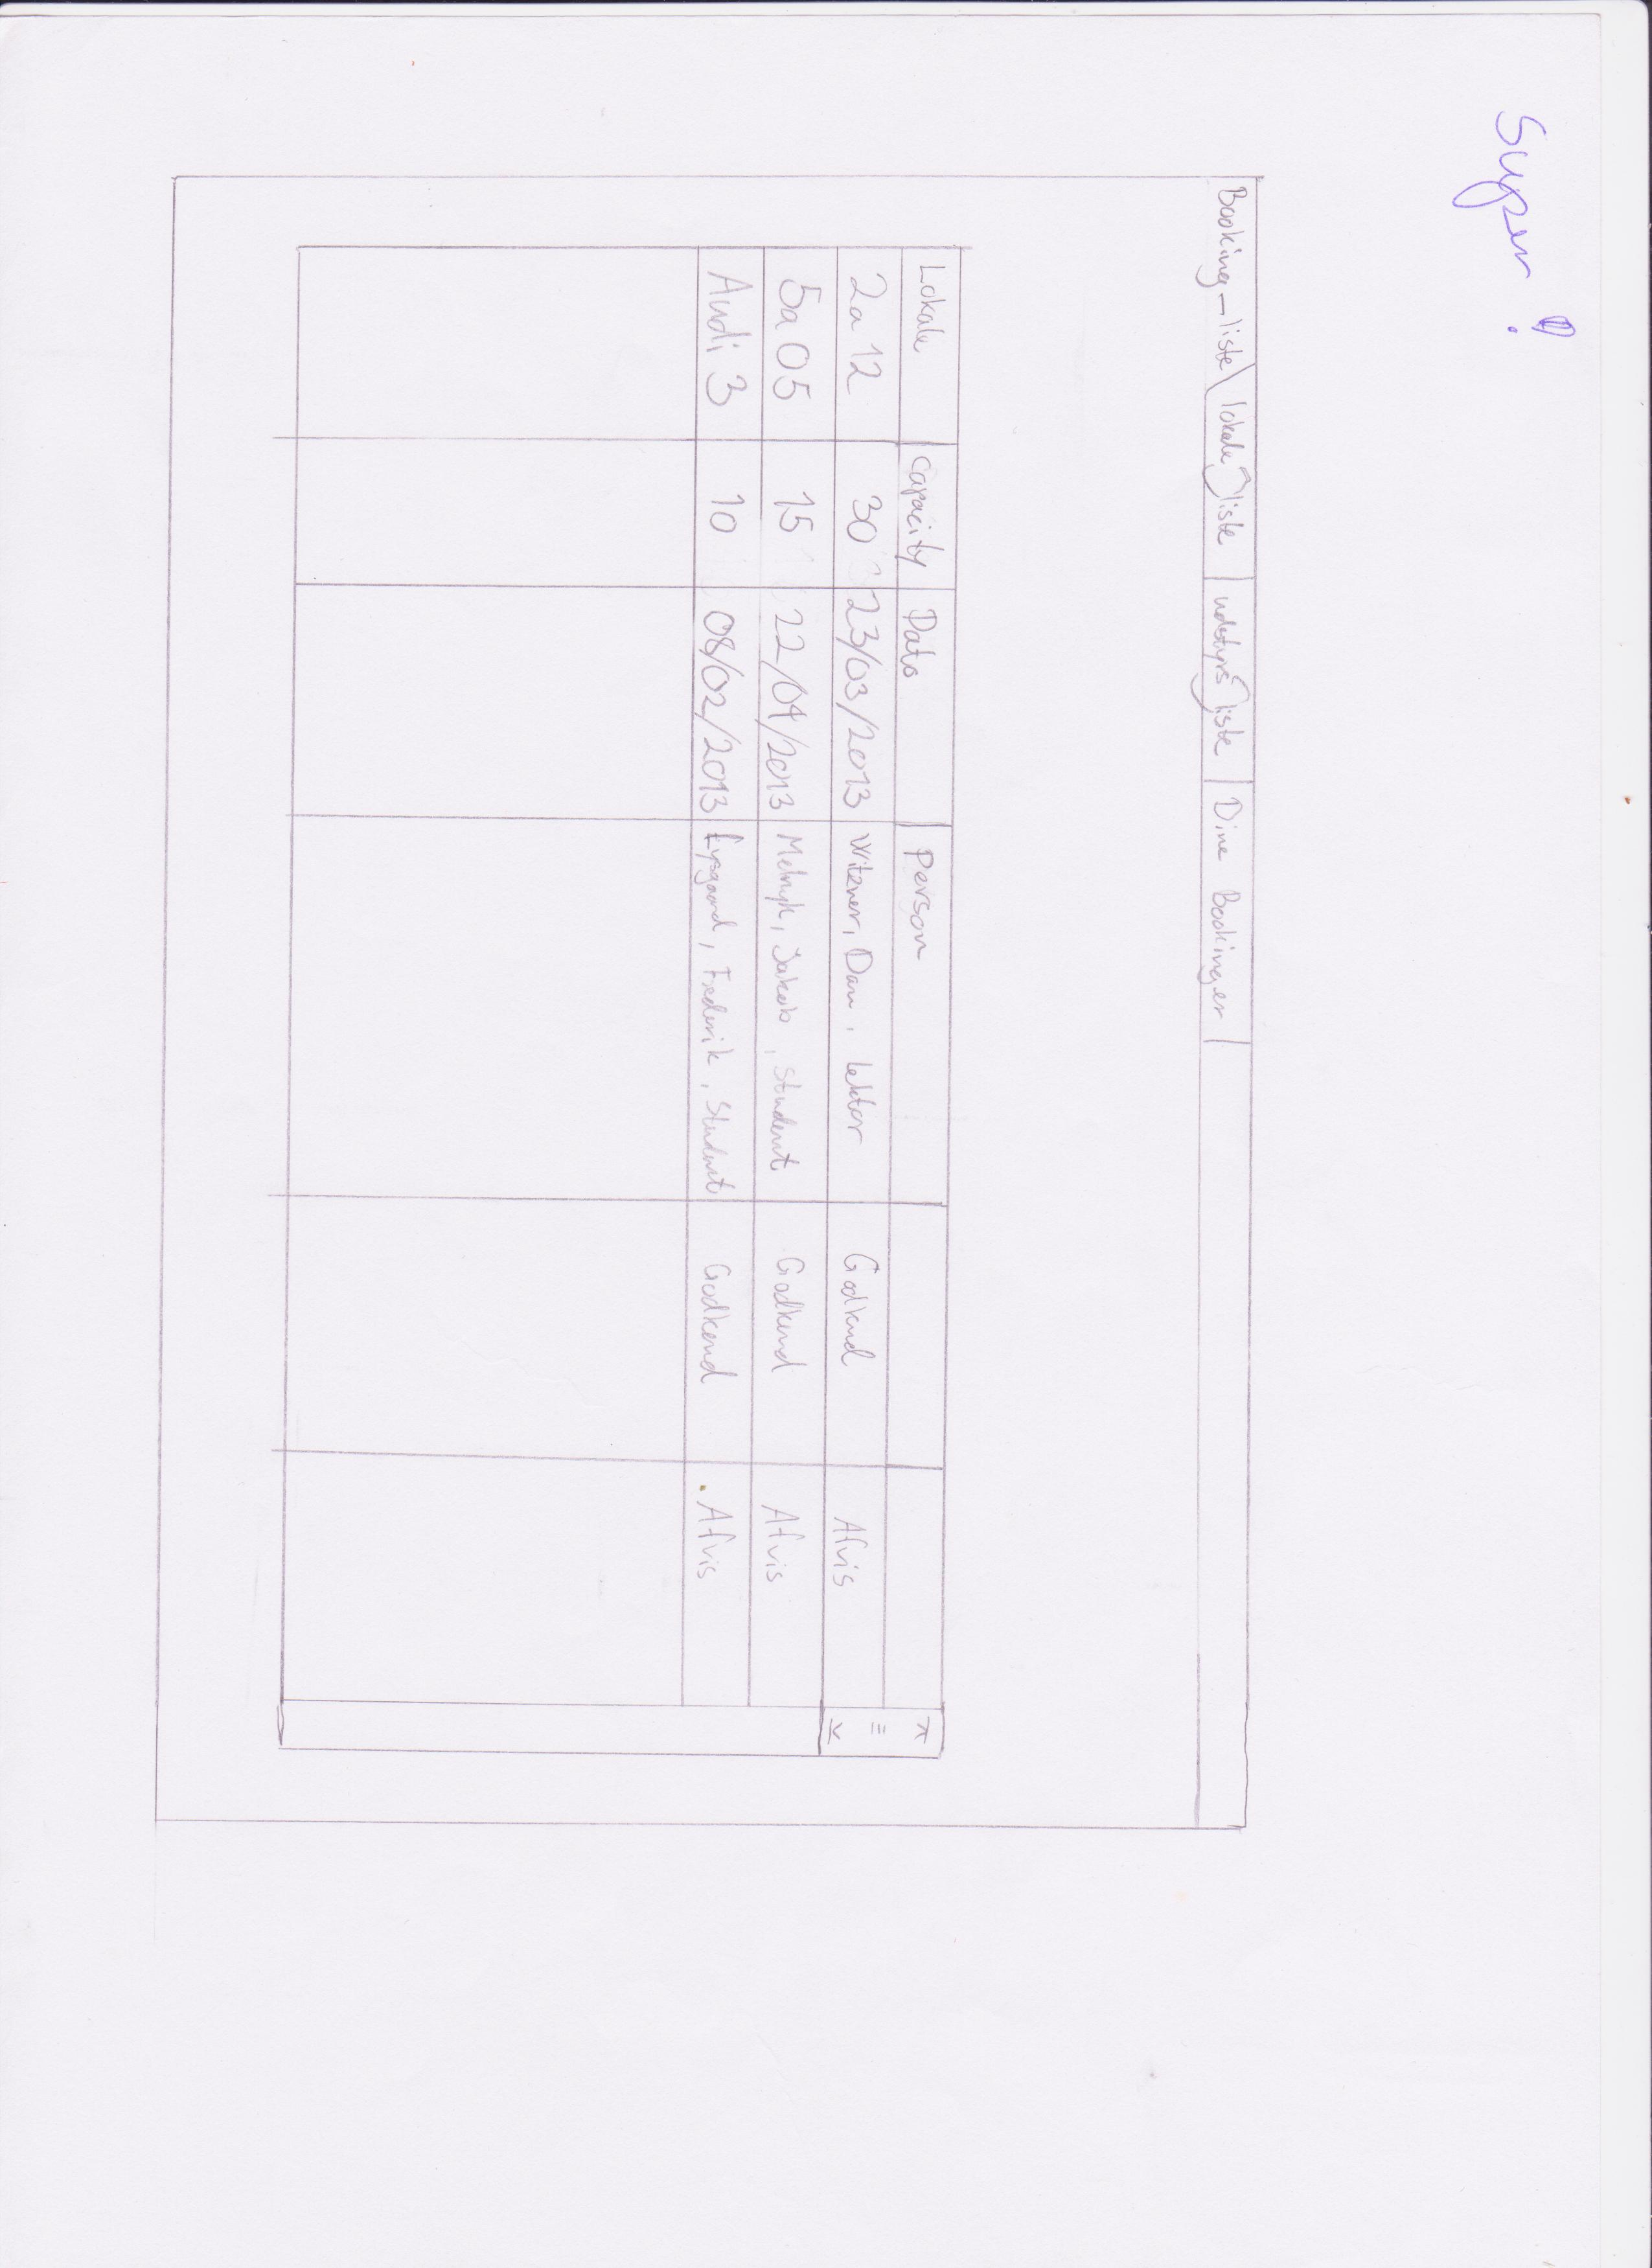
\includegraphics[width=0.7\textwidth]{Appendix/GUI-Prototype/PaperMockup/GodkendBookinger_001}
  \caption{Papermockup af skærmbilledet til godkendelse og afvisning af bookinger}
\label{Design_G_Development_BookingListe}
\end{figure} 

"Booking-liste" skærmbilledet (figur \ref{Design_G_Development_BookingListe_Final}) giver mulighed for at godkende og afvise forespurgte bookinger.
\\Figur \ref{Design_G_Development_BookingListe} viser vores papermockup til skærmbilledet. I papermockuppen havde vi en godkend og afvis knap inde i hver række. Vi besluttede os dog for, at det ville være mere intuitivt, hvis man skulle trykke på en rækker og derefter trykke på et knap uden for gitteret. Derfor flyttede vi "Godkend" og "Afvis" knapperne ned under gitteret.

\subsection{Udstyrsliste}
\begin{figure}[h!]
  \centering
    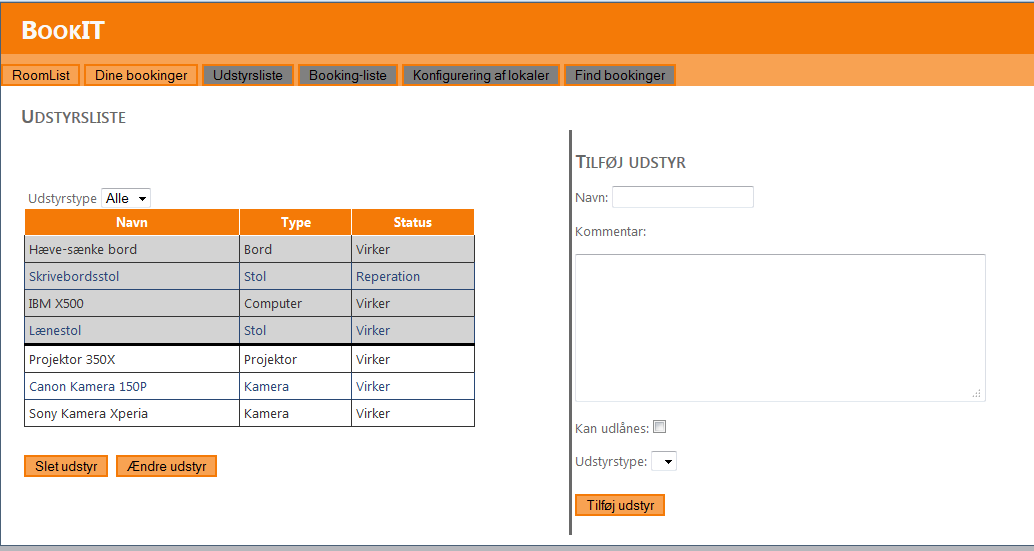
\includegraphics[width=0.9\textwidth]{Appendix/GUI-Prototype/DigitalMockup/UdstyrsListe}
  \caption{Skærmbilledet af receptionistens liste over udstyr i systemet.}
\label{Design_G_Development_UdstyrsListe_Final}
\end{figure} 

Skærmbilledet "Udstyrsliste" (figur \ref{Design_G_Development_UdstyrsListe_Final}) er delt op i to dele. Den venstre del af skærmbilledet er der en liste af inventar og udstyr. Den øverste del af listen (rækker markeret med gråt) er inventar og den nederste del af listen (rækker markeret med hvidt) er udstyr. Den højre side af skærmbilledet giver mulighed for at tilføje udstyr til systemet.

Vi kombinerede overblikket over udstyr og muligheden for at tilføje nyt, fordi vi ville have så få skærmbillederne som muligt uden, at det blev uoverskueligt for brugeren.

Den eneste ændring siden vores papermockup (figur \ref{App_GUI_paper_UdstyrsListe}) er tilføjelsen af en checkboks, hvor man kan vælge det nye udstyr skal være til rådighed for udlån. Da udstyr og inventar er meget ens, så sparer vi et skærmbillede væk ved at kombinere oversigten af de to typer.

Dette betyder, at vi sparer et skærmbillede væk. Da udstyr og inventar er stort set ens i systemet, kan vi afgøre, om det nye element er inventar eller udstyr gennem denne checkbox.

\subsection{Ændring af lokale}
\begin{figure}[h!]
  \centering
    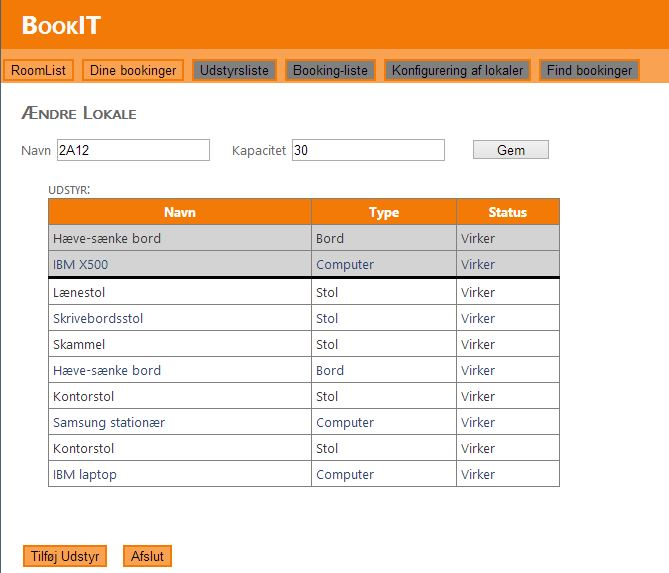
\includegraphics[width=0.8\textwidth]{Appendix/GUI-Prototype/DigitalMockup/AendreLokale}
  \caption{Skærmbilledet til ændring af lokale.}
\label{Design_G_Development_AendreLokale_Final}
\end{figure} 

\begin{figure}[h!]
  \centering
    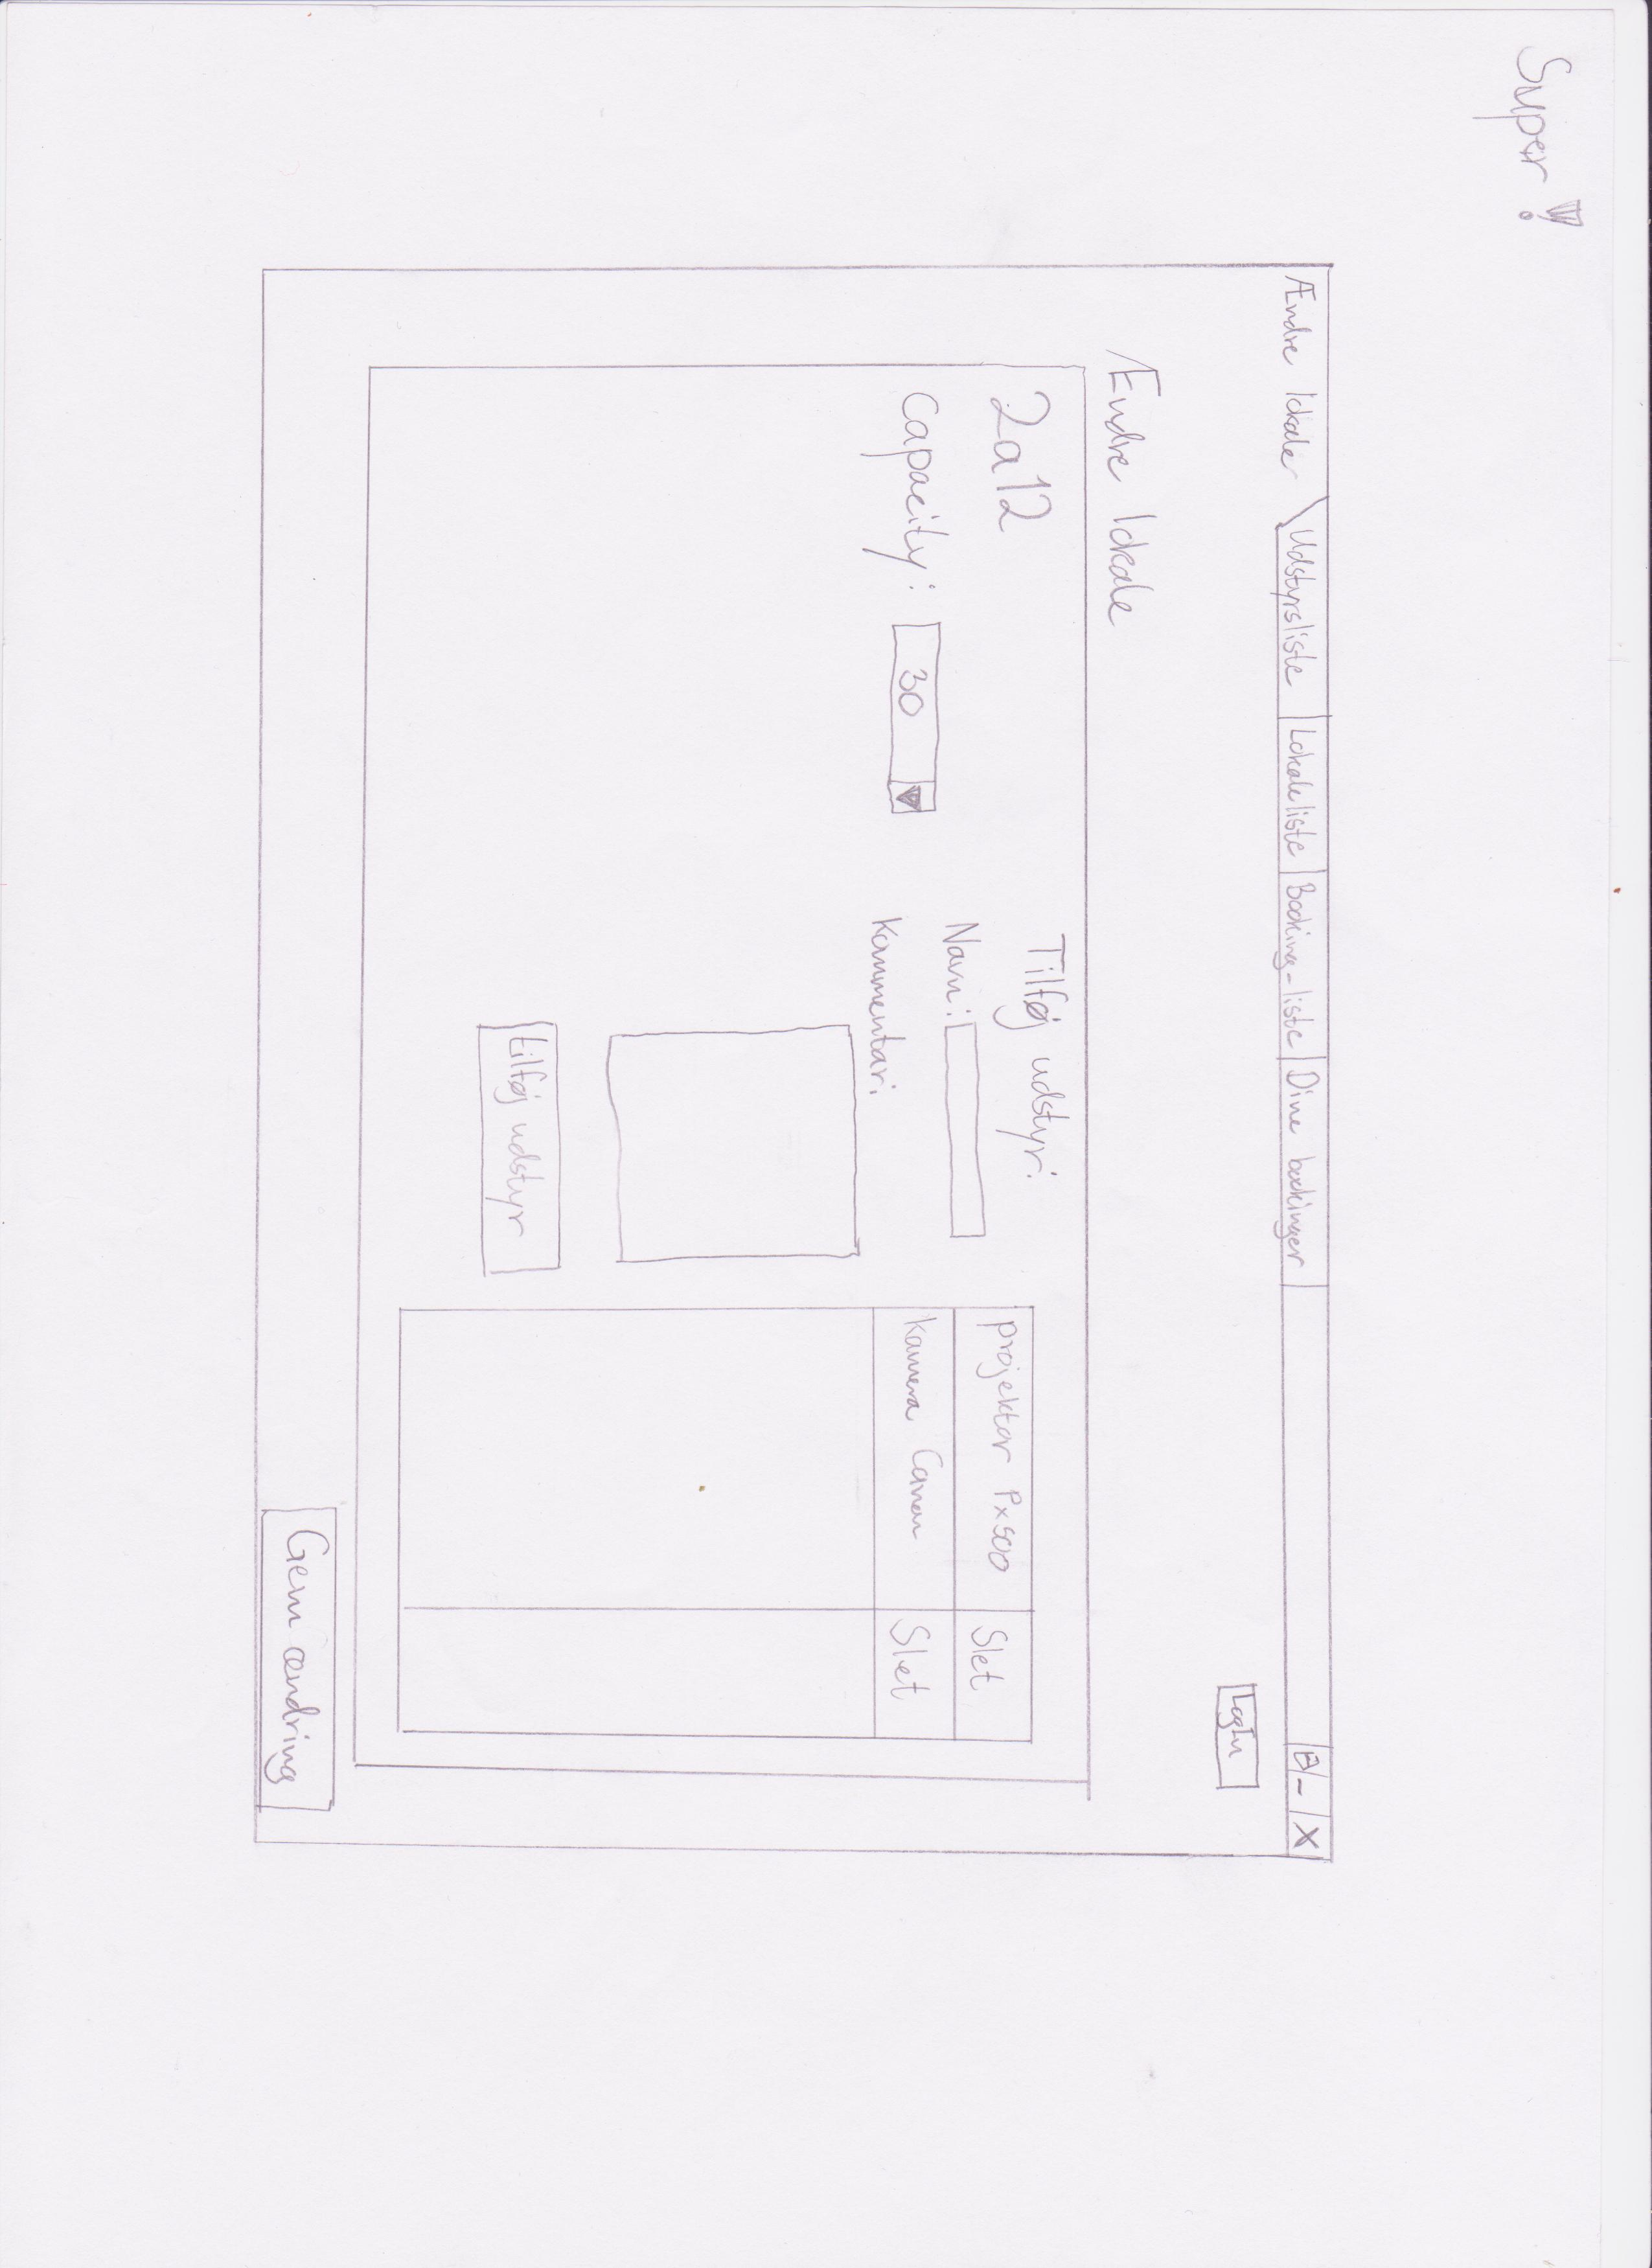
\includegraphics[, width=0.7\textwidth]{Appendix/GUI-Prototype/PaperMockup/AendreLokale_001}
  \caption{Papermockup til ændring af lokale.}
\label{Design_G_Development_AendreLokale}
\end{figure} 
"Ændre lokale" skærmbilledet gør det muligt for administratoren at ændre navn og kapacitet på et lokale. Derudover givet skærmbilledet en oversigt over inventaret, som er tilknyttet lokalet. Den øverste del af listen viser det inventar, som er tilknyttet lokalet, mens den nederste del viser det inventar, som ikke er tilknyttet et lokale.
\\Knappen "Tilføj udstyr" ændrer tekst og funktion an på, om det valgte inventar er tilknyttet lokalet eller ej. Hvis det valgte inventar er tilknyttet lokalet, vil teksten ændre sig til "Fjern Udstyr".

Vores første udkast til skærmbilledet (figur \ref{Design_G_Development_AendreLokale}) var delt i tre: ændring af navn/kapacitet, tilføjelse af udstyr og fjernelse af udstyr. Dette var meget uoverskueligt og mindede ikke om resten af brugergrænsefladen. Vi valgte derfor at anvende samme gitter løsning, som vi har anvendt andre steder i systemet.

\section{Generelle mål}
\label{Design_G_Goals}
Vi har valgt at designe vores brugergrænseflade ud fra reglerne om design af virtuelle vinduer\cite[s. 169]{SL_UID} samt Ease Of Use principperne\cite[s. 9]{SL_UID}. I forbindelse med dette valg har vi sat følgende mål for designet:
\begin{itemize}
\item Konsistent brugergrænseflade
\item Få forskellige skærmbilleder
\item Overblik
\item Effektivt
\end{itemize}

\subsection{Konsistent brugergrænseflade}
Vi har valgt at designe skærmbillederne med samme grundstruktur. Denne lighed bør gøre det intuitivt at gå fra et skærmbillede til et andet i forbindelse med udførsel af opgaver. Desuden følger det reglen om få vindueskabeloner.

\subsection{Kort vej fra en opgave til en anden}
Brugergrænsefladen skal gøre det hurtigt og nemt for brugeren at komme fra en opgave til en anden. Dette skal gøres ved at have få skærmbilleder involvereret i en enkelt task (reglen om få vinduer per opgave).

\subsection{Overblik}
Brugeren skal have mulighed for nemt at danne sig overblik over bookinger, udstyr og forplejning\footnote{Reglen om den nødvendige oversigt af data.}. Derfor skal vi have seperate skærmbilleder, som giver overblik over hver type.

\subsection{Effektivt}
Det skal være effektivt at udføre opgaver for brugere, som anvender systemet ofte.